\documentclass[1p]{elsarticle_modified}
%\bibliographystyle{elsarticle-num}

%\usepackage[colorlinks]{hyperref}
%\usepackage{abbrmath_seonhwa} %\Abb, \Ascr, \Acal ,\Abf, \Afrak
\usepackage{amsfonts}
\usepackage{amssymb}
\usepackage{amsmath}
\usepackage{amsthm}
\usepackage{scalefnt}
\usepackage{amsbsy}
\usepackage{kotex}
\usepackage{caption}
\usepackage{subfig}
\usepackage{color}
\usepackage{graphicx}
\usepackage{xcolor} %% white, black, red, green, blue, cyan, magenta, yellow
\usepackage{float}
\usepackage{setspace}
\usepackage{hyperref}

\usepackage{tikz}
\usetikzlibrary{arrows}

\usepackage{multirow}
\usepackage{array} % fixed length table
\usepackage{hhline}

%%%%%%%%%%%%%%%%%%%%%
\makeatletter
\renewcommand*\env@matrix[1][\arraystretch]{%
	\edef\arraystretch{#1}%
	\hskip -\arraycolsep
	\let\@ifnextchar\new@ifnextchar
	\array{*\c@MaxMatrixCols c}}
\makeatother %https://tex.stackexchange.com/questions/14071/how-can-i-increase-the-line-spacing-in-a-matrix
%%%%%%%%%%%%%%%

\usepackage[normalem]{ulem}

\newcommand{\msout}[1]{\ifmmode\text{\sout{\ensuremath{#1}}}\else\sout{#1}\fi}
%SOURCE: \msout is \stkout macro in https://tex.stackexchange.com/questions/20609/strikeout-in-math-mode

\newcommand{\cancel}[1]{
	\ifmmode
	{\color{red}\msout{#1}}
	\else
	{\color{red}\sout{#1}}
	\fi
}

\newcommand{\add}[1]{
	{\color{blue}\uwave{#1}}
}

\newcommand{\replace}[2]{
	\ifmmode
	{\color{red}\msout{#1}}{\color{blue}\uwave{#2}}
	\else
	{\color{red}\sout{#1}}{\color{blue}\uwave{#2}}
	\fi
}

\newcommand{\Sol}{\mathcal{S}} %segment
\newcommand{\D}{D} %diagram
\newcommand{\A}{\mathcal{A}} %arc


%%%%%%%%%%%%%%%%%%%%%%%%%%%%%5 test

\def\sl{\operatorname{\textup{SL}}(2,\Cbb)}
\def\psl{\operatorname{\textup{PSL}}(2,\Cbb)}
\def\quan{\mkern 1mu \triangleright \mkern 1mu}

\theoremstyle{definition}
\newtheorem{thm}{Theorem}[section]
\newtheorem{prop}[thm]{Proposition}
\newtheorem{lem}[thm]{Lemma}
\newtheorem{ques}[thm]{Question}
\newtheorem{cor}[thm]{Corollary}
\newtheorem{defn}[thm]{Definition}
\newtheorem{exam}[thm]{Example}
\newtheorem{rmk}[thm]{Remark}
\newtheorem{alg}[thm]{Algorithm}

\newcommand{\I}{\sqrt{-1}}
\begin{document}

%\begin{frontmatter}
%
%\title{Boundary parabolic representations of knots up to 8 crossings}
%
%%% Group authors per affiliation:
%\author{Yunhi Cho} 
%\address{Department of Mathematics, University of Seoul, Seoul, Korea}
%\ead{yhcho@uos.ac.kr}
%
%
%\author{Seonhwa Kim} %\fnref{s_kim}}
%\address{Center for Geometry and Physics, Institute for Basic Science, Pohang, 37673, Korea}
%\ead{ryeona17@ibs.re.kr}
%
%\author{Hyuk Kim}
%\address{Department of Mathematical Sciences, Seoul National University, Seoul 08826, Korea}
%\ead{hyukkim@snu.ac.kr}
%
%\author{Seokbeom Yoon}
%\address{Department of Mathematical Sciences, Seoul National University, Seoul, 08826,  Korea}
%\ead{sbyoon15@snu.ac.kr}
%
%\begin{abstract}
%We find all boundary parabolic representation of knots up to 8 crossings.
%
%\end{abstract}
%\begin{keyword}
%    \MSC[2010] 57M25 
%\end{keyword}
%
%\end{frontmatter}

%\linenumbers
%\tableofcontents
%
\newcommand\colored[1]{\textcolor{white}{\rule[-0.35ex]{0.8em}{1.4ex}}\kern-0.8em\color{red} #1}%
%\newcommand\colored[1]{\textcolor{white}{ #1}\kern-2.17ex	\textcolor{white}{ #1}\kern-1.81ex	\textcolor{white}{ #1}\kern-2.15ex\color{red}#1	}

{\Large $\underline{12a_{0307}~(K12a_{0307})}$}

\setlength{\tabcolsep}{10pt}
\renewcommand{\arraystretch}{1.6}
\vspace{1cm}\begin{tabular}{m{100pt}>{\centering\arraybackslash}m{274pt}}
\multirow{5}{120pt}{
	\centering
	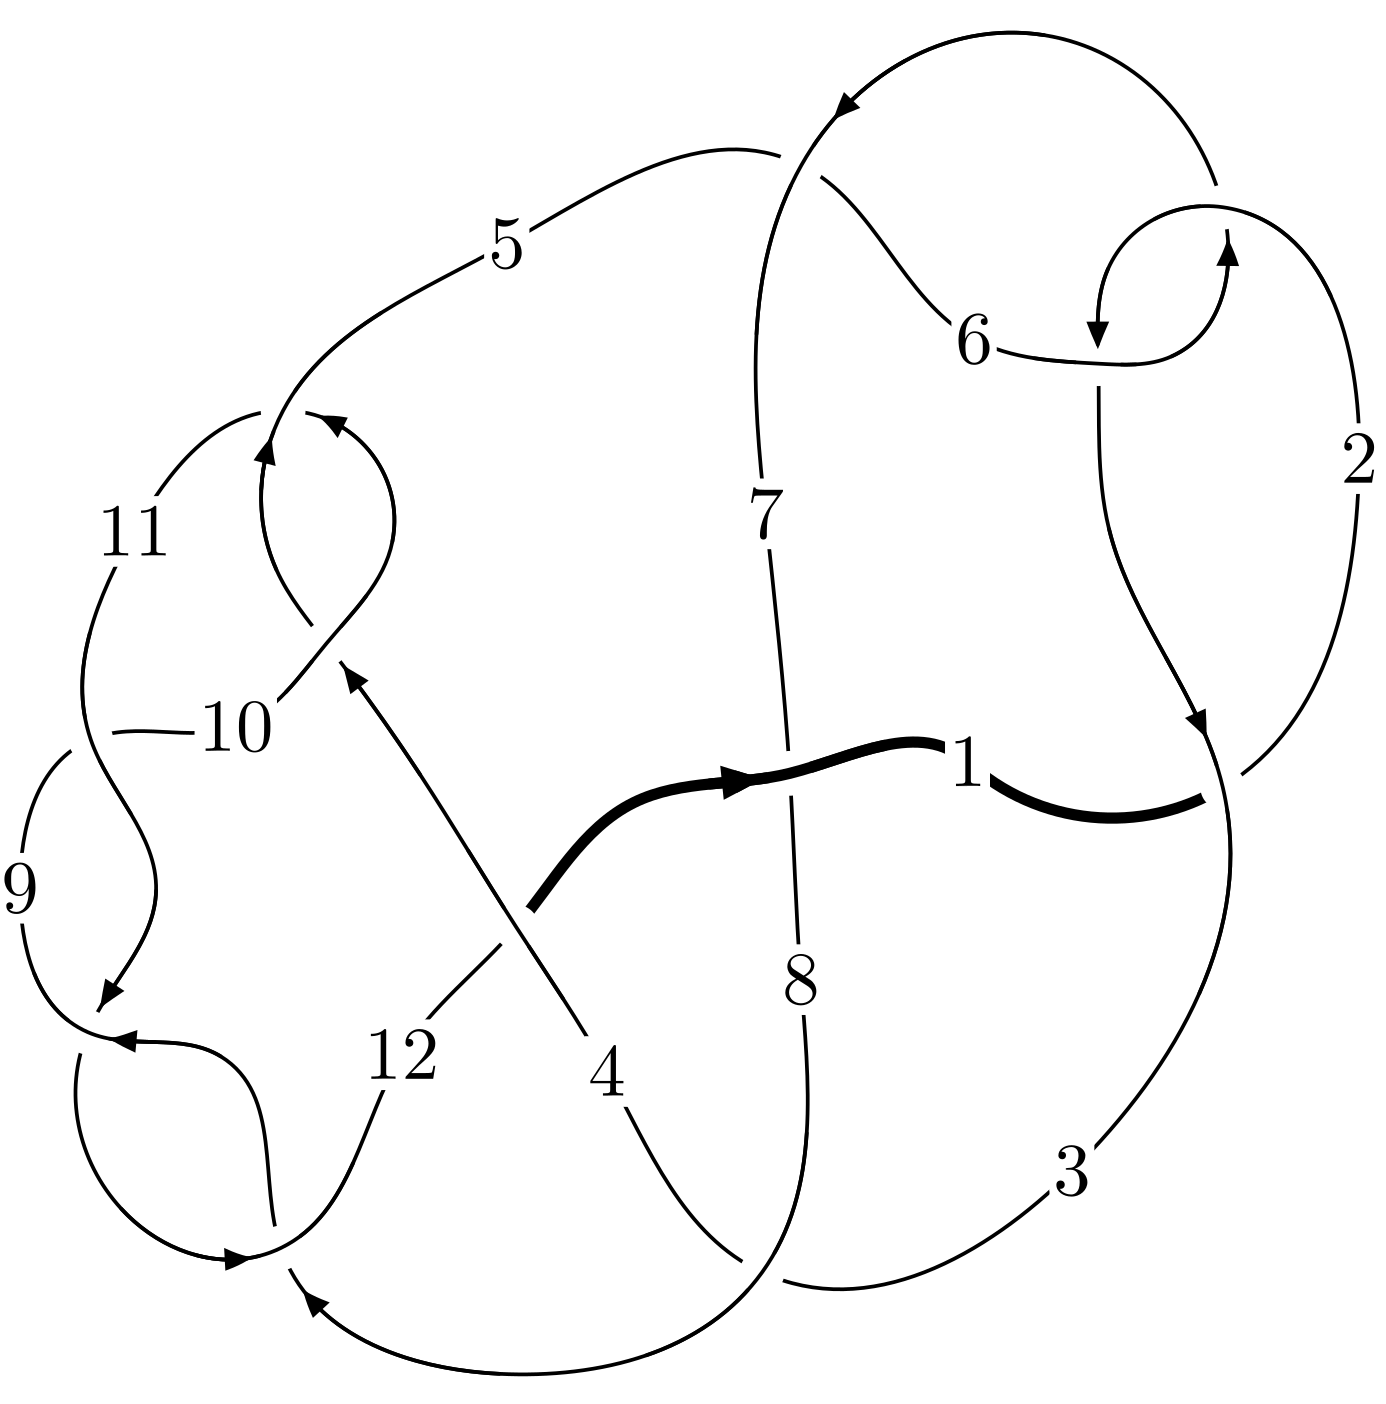
\includegraphics[width=112pt]{../../../GIT/diagram.site/Diagrams/png/1108_12a_0307.png}\\
\ \ \ A knot diagram\footnotemark}&
\allowdisplaybreaks
\textbf{Linearized knot diagam} \\
\cline{2-2}
 &
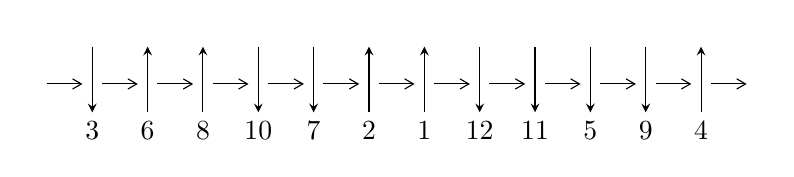
\begin{tikzpicture}[x=20pt, y=17pt]
	% nodes
	\node (C0) at (0, 0) {};
	\node (C1) at (1, 0) {};
	\node (C1U) at (1, +1) {};
	\node (C1D) at (1, -1) {3};

	\node (C2) at (2, 0) {};
	\node (C2U) at (2, +1) {};
	\node (C2D) at (2, -1) {6};

	\node (C3) at (3, 0) {};
	\node (C3U) at (3, +1) {};
	\node (C3D) at (3, -1) {8};

	\node (C4) at (4, 0) {};
	\node (C4U) at (4, +1) {};
	\node (C4D) at (4, -1) {10};

	\node (C5) at (5, 0) {};
	\node (C5U) at (5, +1) {};
	\node (C5D) at (5, -1) {7};

	\node (C6) at (6, 0) {};
	\node (C6U) at (6, +1) {};
	\node (C6D) at (6, -1) {2};

	\node (C7) at (7, 0) {};
	\node (C7U) at (7, +1) {};
	\node (C7D) at (7, -1) {1};

	\node (C8) at (8, 0) {};
	\node (C8U) at (8, +1) {};
	\node (C8D) at (8, -1) {12};

	\node (C9) at (9, 0) {};
	\node (C9U) at (9, +1) {};
	\node (C9D) at (9, -1) {11};

	\node (C10) at (10, 0) {};
	\node (C10U) at (10, +1) {};
	\node (C10D) at (10, -1) {5};

	\node (C11) at (11, 0) {};
	\node (C11U) at (11, +1) {};
	\node (C11D) at (11, -1) {9};

	\node (C12) at (12, 0) {};
	\node (C12U) at (12, +1) {};
	\node (C12D) at (12, -1) {4};
	\node (C13) at (13, 0) {};

	% arrows
	\draw[->,>={angle 60}]
	(C0) edge (C1) (C1) edge (C2) (C2) edge (C3) (C3) edge (C4) (C4) edge (C5) (C5) edge (C6) (C6) edge (C7) (C7) edge (C8) (C8) edge (C9) (C9) edge (C10) (C10) edge (C11) (C11) edge (C12) (C12) edge (C13) ;	\draw[->,>=stealth]
	(C1U) edge (C1D) (C2D) edge (C2U) (C3D) edge (C3U) (C4U) edge (C4D) (C5U) edge (C5D) (C6D) edge (C6U) (C7D) edge (C7U) (C8U) edge (C8D) (C9U) edge (C9D) (C10U) edge (C10D) (C11U) edge (C11D) (C12D) edge (C12U) ;
	\end{tikzpicture} \\
\hhline{~~} \\& 
\textbf{Solving Sequence} \\ \cline{2-2} 
 &
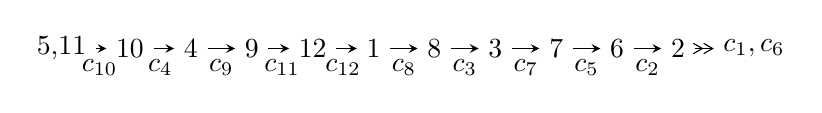
\begin{tikzpicture}[x=22pt, y=7pt]
	% node
	\node (A0) at (-1/8, 0) {5,11};
	\node (A1) at (1, 0) {10};
	\node (A2) at (2, 0) {4};
	\node (A3) at (3, 0) {9};
	\node (A4) at (4, 0) {12};
	\node (A5) at (5, 0) {1};
	\node (A6) at (6, 0) {8};
	\node (A7) at (7, 0) {3};
	\node (A8) at (8, 0) {7};
	\node (A9) at (9, 0) {6};
	\node (A10) at (10, 0) {2};
	\node (C1) at (1/2, -1) {$c_{10}$};
	\node (C2) at (3/2, -1) {$c_{4}$};
	\node (C3) at (5/2, -1) {$c_{9}$};
	\node (C4) at (7/2, -1) {$c_{11}$};
	\node (C5) at (9/2, -1) {$c_{12}$};
	\node (C6) at (11/2, -1) {$c_{8}$};
	\node (C7) at (13/2, -1) {$c_{3}$};
	\node (C8) at (15/2, -1) {$c_{7}$};
	\node (C9) at (17/2, -1) {$c_{5}$};
	\node (C10) at (19/2, -1) {$c_{2}$};
	\node (A11) at (45/4, 0) {$c_{1},c_{6}$};

	% edge
	\draw[->,>=stealth]	
	(A0) edge (A1) (A1) edge (A2) (A2) edge (A3) (A3) edge (A4) (A4) edge (A5) (A5) edge (A6) (A6) edge (A7) (A7) edge (A8) (A8) edge (A9) (A9) edge (A10) ;
	\draw[->>,>={angle 60}]	
	(A10) edge (A11);
\end{tikzpicture} \\ 

\end{tabular} \\

\footnotetext{
The image of knot diagram is generated by the software ``\textbf{Draw programme}" developed by Andrew Bartholomew(\url{http://www.layer8.co.uk/maths/draw/index.htm\#Running-draw}), where we modified some parts for our purpose(\url{https://github.com/CATsTAILs/LinksPainter}).
}\phantom \\ \newline 
\centering \textbf{Ideals for irreducible components\footnotemark of $X_{\text{par}}$} 
 
\begin{align*}
I^u_{1}&=\langle 
u^{78}+u^{77}+\cdots- u+1\rangle \\
\\
\end{align*}
\raggedright * 1 irreducible components of $\dim_{\mathbb{C}}=0$, with total 78 representations.\\
\footnotetext{All coefficients of polynomials are rational numbers. But the coefficients are sometimes approximated in decimal forms when there is not enough margin.}
\newpage
\renewcommand{\arraystretch}{1}
\centering \section*{I. $I^u_{1}= \langle u^{78}+u^{77}+\cdots- u+1 \rangle$}
\flushleft \textbf{(i) Arc colorings}\\
\begin{tabular}{m{7pt} m{180pt} m{7pt} m{180pt} }
\flushright $a_{5}=$&$\begin{pmatrix}0\\u\end{pmatrix}$ \\
\flushright $a_{11}=$&$\begin{pmatrix}1\\0\end{pmatrix}$ \\
\flushright $a_{10}=$&$\begin{pmatrix}1\\- u^2\end{pmatrix}$ \\
\flushright $a_{4}=$&$\begin{pmatrix}u\\- u^3+u\end{pmatrix}$ \\
\flushright $a_{9}=$&$\begin{pmatrix}- u^2+1\\- u^2\end{pmatrix}$ \\
\flushright $a_{12}=$&$\begin{pmatrix}u^4- u^2+1\\u^4\end{pmatrix}$ \\
\flushright $a_{1}=$&$\begin{pmatrix}u^8- u^6+3 u^4-2 u^2+1\\- u^{10}+2 u^8-3 u^6+4 u^4- u^2\end{pmatrix}$ \\
\flushright $a_{8}=$&$\begin{pmatrix}- u^6+u^4-2 u^2+1\\- u^6- u^2\end{pmatrix}$ \\
\flushright $a_{3}=$&$\begin{pmatrix}u^{15}-2 u^{13}+6 u^{11}-8 u^9+10 u^7-8 u^5+4 u^3\\u^{15}- u^{13}+4 u^{11}-3 u^9+4 u^7-2 u^5+u\end{pmatrix}$ \\
\flushright $a_{7}=$&$\begin{pmatrix}u^{24}-3 u^{22}+\cdots-2 u^2+1\\- u^{26}+4 u^{24}+\cdots-5 u^6- u^2\end{pmatrix}$ \\
\flushright $a_{6}=$&$\begin{pmatrix}- u^{49}+6 u^{47}+\cdots+4 u^3- u\\u^{51}-7 u^{49}+\cdots+u^3+u\end{pmatrix}$ \\
\flushright $a_{2}=$&$\begin{pmatrix}u^{40}-5 u^{38}+\cdots-2 u^2+1\\u^{40}-4 u^{38}+\cdots-7 u^8+2 u^4\end{pmatrix}$\\&\end{tabular}
\flushleft \textbf{(ii) Obstruction class $= -1$}\\~\\
\flushleft \textbf{(iii) Cusp Shapes $= 4 u^{76}+4 u^{75}+\cdots+4 u-6$}\\~\\
\newpage\renewcommand{\arraystretch}{1}
\flushleft \textbf{(iv) u-Polynomials at the component}\newline \\
\begin{tabular}{m{50pt}|m{274pt}}
Crossings & \hspace{64pt}u-Polynomials at each crossing \\
\hline $$\begin{aligned}c_{1},c_{5}\end{aligned}$$&$\begin{aligned}
&u^{78}+25 u^{77}+\cdots- u+1
\end{aligned}$\\
\hline $$\begin{aligned}c_{2},c_{6}\end{aligned}$$&$\begin{aligned}
&u^{78}- u^{77}+\cdots+u+1
\end{aligned}$\\
\hline $$\begin{aligned}c_{3}\end{aligned}$$&$\begin{aligned}
&u^{78}- u^{77}+\cdots+12563 u+3361
\end{aligned}$\\
\hline $$\begin{aligned}c_{4},c_{10}\end{aligned}$$&$\begin{aligned}
&u^{78}- u^{77}+\cdots+u+1
\end{aligned}$\\
\hline $$\begin{aligned}c_{7}\end{aligned}$$&$\begin{aligned}
&u^{78}+5 u^{77}+\cdots+13 u+3
\end{aligned}$\\
\hline $$\begin{aligned}c_{8},c_{9},c_{11}\end{aligned}$$&$\begin{aligned}
&u^{78}+19 u^{77}+\cdots+u+1
\end{aligned}$\\
\hline $$\begin{aligned}c_{12}\end{aligned}$$&$\begin{aligned}
&u^{78}+7 u^{77}+\cdots+101 u+391
\end{aligned}$\\
\hline
\end{tabular}\\~\\
\newpage\renewcommand{\arraystretch}{1}
\flushleft \textbf{(v) Riley Polynomials at the component}\newline \\
\begin{tabular}{m{50pt}|m{274pt}}
Crossings & \hspace{64pt}Riley Polynomials at each crossing \\
\hline $$\begin{aligned}c_{1},c_{5}\end{aligned}$$&$\begin{aligned}
&y^{78}+57 y^{77}+\cdots- y+1
\end{aligned}$\\
\hline $$\begin{aligned}c_{2},c_{6}\end{aligned}$$&$\begin{aligned}
&y^{78}+25 y^{77}+\cdots- y+1
\end{aligned}$\\
\hline $$\begin{aligned}c_{3}\end{aligned}$$&$\begin{aligned}
&y^{78}-31 y^{77}+\cdots-206603801 y+11296321
\end{aligned}$\\
\hline $$\begin{aligned}c_{4},c_{10}\end{aligned}$$&$\begin{aligned}
&y^{78}-19 y^{77}+\cdots- y+1
\end{aligned}$\\
\hline $$\begin{aligned}c_{7}\end{aligned}$$&$\begin{aligned}
&y^{78}-3 y^{77}+\cdots+347 y+9
\end{aligned}$\\
\hline $$\begin{aligned}c_{8},c_{9},c_{11}\end{aligned}$$&$\begin{aligned}
&y^{78}+81 y^{77}+\cdots+7 y+1
\end{aligned}$\\
\hline $$\begin{aligned}c_{12}\end{aligned}$$&$\begin{aligned}
&y^{78}-11 y^{77}+\cdots-1417801 y+152881
\end{aligned}$\\
\hline
\end{tabular}\\~\\
\newpage\flushleft \textbf{(vi) Complex Volumes and Cusp Shapes}
$$\begin{array}{c|c|c}  
\text{Solutions to }I^u_{1}& \I (\text{vol} + \sqrt{-1}CS) & \text{Cusp shape}\\
 \hline 
\begin{aligned}
u &= \phantom{-}0.949193 + 0.358040 I\end{aligned}
 & -4.26149 - 6.00568 I & \phantom{-0.000000 } 0 \\ \hline\begin{aligned}
u &= \phantom{-}0.949193 - 0.358040 I\end{aligned}
 & -4.26149 + 6.00568 I & \phantom{-0.000000 } 0 \\ \hline\begin{aligned}
u &= -0.909376 + 0.367190 I\end{aligned}
 & -0.50435 + 3.91121 I & \phantom{-0.000000 } 0. - 7.54599 I \\ \hline\begin{aligned}
u &= -0.909376 - 0.367190 I\end{aligned}
 & -0.50435 - 3.91121 I & \phantom{-0.000000 -}0. + 7.54599 I \\ \hline\begin{aligned}
u &= \phantom{-}0.922832 + 0.301327 I\end{aligned}
 & -2.15865 - 0.42474 I & -6.89852 + 0. I\phantom{ +0.000000I} \\ \hline\begin{aligned}
u &= \phantom{-}0.922832 - 0.301327 I\end{aligned}
 & -2.15865 + 0.42474 I & -6.89852 + 0. I\phantom{ +0.000000I} \\ \hline\begin{aligned}
u &= -0.953974 + 0.390613 I\end{aligned}
 & \phantom{-}2.02865 + 5.81503 I & \phantom{-0.000000 } 0 \\ \hline\begin{aligned}
u &= -0.953974 - 0.390613 I\end{aligned}
 & \phantom{-}2.02865 - 5.81503 I & \phantom{-0.000000 } 0 \\ \hline\begin{aligned}
u &= -0.853626 + 0.453737 I\end{aligned}
 & \phantom{-}3.50897 + 3.53165 I & \phantom{-0.000000 } 0. - 6.38769 I \\ \hline\begin{aligned}
u &= -0.853626 - 0.453737 I\end{aligned}
 & \phantom{-}3.50897 - 3.53165 I & \phantom{-0.000000 -}0. + 6.38769 I \\ \hline\begin{aligned}
u &= \phantom{-}0.963013 + 0.386433 I\end{aligned}
 & \phantom{-}1.09694 - 11.54900 I & \phantom{-0.000000 } 0 \\ \hline\begin{aligned}
u &= \phantom{-}0.963013 - 0.386433 I\end{aligned}
 & \phantom{-}1.09694 + 11.54900 I & \phantom{-0.000000 } 0 \\ \hline\begin{aligned}
u &= -0.925410 + 0.238058 I\end{aligned}
 & -2.50131 + 4.74725 I & -7.86723 - 7.24830 I \\ \hline\begin{aligned}
u &= -0.925410 - 0.238058 I\end{aligned}
 & -2.50131 - 4.74725 I & -7.86723 + 7.24830 I \\ \hline\begin{aligned}
u &= \phantom{-}0.826172 + 0.475093 I\end{aligned}
 & \phantom{-}3.01816 + 2.08322 I & \phantom{-0.000000 } 0 \\ \hline\begin{aligned}
u &= \phantom{-}0.826172 - 0.475093 I\end{aligned}
 & \phantom{-}3.01816 - 2.08322 I & \phantom{-0.000000 } 0 \\ \hline\begin{aligned}
u &= -0.936652 + 0.113686 I\end{aligned}
 & -0.43311 - 6.13558 I & -5.92020 + 4.39204 I \\ \hline\begin{aligned}
u &= -0.936652 - 0.113686 I\end{aligned}
 & -0.43311 + 6.13558 I & -5.92020 - 4.39204 I \\ \hline\begin{aligned}
u &= -0.921742 + 0.168035 I\end{aligned}
 & -5.33588 - 0.72951 I & -12.03847 + 0. I\phantom{ +0.000000I} \\ \hline\begin{aligned}
u &= -0.921742 - 0.168035 I\end{aligned}
 & -5.33588 + 0.72951 I & -12.03847 + 0. I\phantom{ +0.000000I} \\ \hline\begin{aligned}
u &= \phantom{-}0.918147 + 0.102714 I\end{aligned}
 & \phantom{-}0.436101 + 0.552797 I & -4.23323 + 0.60202 I \\ \hline\begin{aligned}
u &= \phantom{-}0.918147 - 0.102714 I\end{aligned}
 & \phantom{-}0.436101 - 0.552797 I & -4.23323 - 0.60202 I \\ \hline\begin{aligned}
u &= \phantom{-}0.837889 + 0.209909 I\end{aligned}
 & -1.48994 - 0.67769 I & -4.74017 + 0.61730 I \\ \hline\begin{aligned}
u &= \phantom{-}0.837889 - 0.209909 I\end{aligned}
 & -1.48994 + 0.67769 I & -4.74017 - 0.61730 I \\ \hline\begin{aligned}
u &= \phantom{-}0.846308 + 0.782773 I\end{aligned}
 & \phantom{-}3.69266 + 2.68084 I & \phantom{-0.000000 } 0 \\ \hline\begin{aligned}
u &= \phantom{-}0.846308 - 0.782773 I\end{aligned}
 & \phantom{-}3.69266 - 2.68084 I & \phantom{-0.000000 } 0 \\ \hline\begin{aligned}
u &= \phantom{-}0.891675 + 0.767032 I\end{aligned}
 & -0.21663 - 2.90039 I & \phantom{-0.000000 } 0 \\ \hline\begin{aligned}
u &= \phantom{-}0.891675 - 0.767032 I\end{aligned}
 & -0.21663 + 2.90039 I & \phantom{-0.000000 } 0 \\ \hline\begin{aligned}
u &= -0.864820 + 0.805829 I\end{aligned}
 & \phantom{-}4.66036 + 2.29542 I & \phantom{-0.000000 } 0 \\ \hline\begin{aligned}
u &= -0.864820 - 0.805829 I\end{aligned}
 & \phantom{-}4.66036 - 2.29542 I & \phantom{-0.000000 } 0\\
 \hline 
 \end{array}$$\newpage$$\begin{array}{c|c|c}  
\text{Solutions to }I^u_{1}& \I (\text{vol} + \sqrt{-1}CS) & \text{Cusp shape}\\
 \hline 
\begin{aligned}
u &= -0.852900 + 0.845500 I\end{aligned}
 & \phantom{-}4.93566 + 2.14676 I & \phantom{-0.000000 } 0 \\ \hline\begin{aligned}
u &= -0.852900 - 0.845500 I\end{aligned}
 & \phantom{-}4.93566 - 2.14676 I & \phantom{-0.000000 } 0 \\ \hline\begin{aligned}
u &= -0.834187 + 0.868906 I\end{aligned}
 & \phantom{-}3.57453 - 3.66845 I & \phantom{-0.000000 } 0 \\ \hline\begin{aligned}
u &= -0.834187 - 0.868906 I\end{aligned}
 & \phantom{-}3.57453 + 3.66845 I & \phantom{-0.000000 } 0 \\ \hline\begin{aligned}
u &= \phantom{-}0.927507 + 0.775603 I\end{aligned}
 & \phantom{-}3.44668 - 8.56088 I & \phantom{-0.000000 } 0 \\ \hline\begin{aligned}
u &= \phantom{-}0.927507 - 0.775603 I\end{aligned}
 & \phantom{-}3.44668 + 8.56088 I & \phantom{-0.000000 } 0 \\ \hline\begin{aligned}
u &= \phantom{-}0.848176 + 0.867614 I\end{aligned}
 & \phantom{-}7.28261 + 1.17492 I & \phantom{-0.000000 } 0 \\ \hline\begin{aligned}
u &= \phantom{-}0.848176 - 0.867614 I\end{aligned}
 & \phantom{-}7.28261 - 1.17492 I & \phantom{-0.000000 } 0 \\ \hline\begin{aligned}
u &= -0.834616 + 0.882587 I\end{aligned}
 & \phantom{-}9.27923 - 9.22489 I & \phantom{-0.000000 } 0 \\ \hline\begin{aligned}
u &= -0.834616 - 0.882587 I\end{aligned}
 & \phantom{-}9.27923 + 9.22489 I & \phantom{-0.000000 } 0 \\ \hline\begin{aligned}
u &= -0.918757 + 0.796116 I\end{aligned}
 & \phantom{-}4.49717 + 3.71365 I & \phantom{-0.000000 } 0 \\ \hline\begin{aligned}
u &= -0.918757 - 0.796116 I\end{aligned}
 & \phantom{-}4.49717 - 3.71365 I & \phantom{-0.000000 } 0 \\ \hline\begin{aligned}
u &= \phantom{-}0.838397 + 0.881767 I\end{aligned}
 & \phantom{-}10.20570 + 3.38686 I & \phantom{-0.000000 } 0 \\ \hline\begin{aligned}
u &= \phantom{-}0.838397 - 0.881767 I\end{aligned}
 & \phantom{-}10.20570 - 3.38686 I & \phantom{-0.000000 } 0 \\ \hline\begin{aligned}
u &= \phantom{-}0.870546 + 0.874779 I\end{aligned}
 & \phantom{-}11.65370 + 0.03173 I & \phantom{-0.000000 } 0 \\ \hline\begin{aligned}
u &= \phantom{-}0.870546 - 0.874779 I\end{aligned}
 & \phantom{-}11.65370 - 0.03173 I & \phantom{-0.000000 } 0 \\ \hline\begin{aligned}
u &= -0.875907 + 0.873132 I\end{aligned}
 & \phantom{-}11.14380 + 5.82310 I & \phantom{-0.000000 } 0 \\ \hline\begin{aligned}
u &= -0.875907 - 0.873132 I\end{aligned}
 & \phantom{-}11.14380 - 5.82310 I & \phantom{-0.000000 } 0 \\ \hline\begin{aligned}
u &= \phantom{-}0.466979 + 0.592674 I\end{aligned}
 & \phantom{-}4.13801 - 6.03877 I & \phantom{-}4.19257 + 6.32156 I \\ \hline\begin{aligned}
u &= \phantom{-}0.466979 - 0.592674 I\end{aligned}
 & \phantom{-}4.13801 + 6.03877 I & \phantom{-}4.19257 - 6.32156 I \\ \hline\begin{aligned}
u &= -0.947419 + 0.811987 I\end{aligned}
 & \phantom{-}4.63904 + 4.03273 I & \phantom{-0.000000 } 0 \\ \hline\begin{aligned}
u &= -0.947419 - 0.811987 I\end{aligned}
 & \phantom{-}4.63904 - 4.03273 I & \phantom{-0.000000 } 0 \\ \hline\begin{aligned}
u &= \phantom{-}0.959984 + 0.824037 I\end{aligned}
 & \phantom{-}6.93085 - 7.45769 I & \phantom{-0.000000 } 0 \\ \hline\begin{aligned}
u &= \phantom{-}0.959984 - 0.824037 I\end{aligned}
 & \phantom{-}6.93085 + 7.45769 I & \phantom{-0.000000 } 0 \\ \hline\begin{aligned}
u &= -0.438234 + 0.587846 I\end{aligned}
 & \phantom{-}4.79894 + 0.34084 I & \phantom{-}5.80799 - 0.75958 I \\ \hline\begin{aligned}
u &= -0.438234 - 0.587846 I\end{aligned}
 & \phantom{-}4.79894 - 0.34084 I & \phantom{-}5.80799 + 0.75958 I \\ \hline\begin{aligned}
u &= -0.945617 + 0.843775 I\end{aligned}
 & \phantom{-}10.92280 + 0.54088 I & \phantom{-0.000000 } 0 \\ \hline\begin{aligned}
u &= -0.945617 - 0.843775 I\end{aligned}
 & \phantom{-}10.92280 - 0.54088 I & \phantom{-0.000000 } 0 \\ \hline\begin{aligned}
u &= -0.968614 + 0.817587 I\end{aligned}
 & \phantom{-}3.15301 + 9.93293 I & \phantom{-0.000000 } 0 \\ \hline\begin{aligned}
u &= -0.968614 - 0.817587 I\end{aligned}
 & \phantom{-}3.15301 - 9.93293 I & \phantom{-0.000000 } 0\\
 \hline 
 \end{array}$$\newpage$$\begin{array}{c|c|c}  
\text{Solutions to }I^u_{1}& \I (\text{vol} + \sqrt{-1}CS) & \text{Cusp shape}\\
 \hline 
\begin{aligned}
u &= \phantom{-}0.950142 + 0.841515 I\end{aligned}
 & \phantom{-}11.40160 - 6.39346 I & \phantom{-0.000000 } 0 \\ \hline\begin{aligned}
u &= \phantom{-}0.950142 - 0.841515 I\end{aligned}
 & \phantom{-}11.40160 + 6.39346 I & \phantom{-0.000000 } 0 \\ \hline\begin{aligned}
u &= \phantom{-}0.973193 + 0.826698 I\end{aligned}
 & \phantom{-}9.78039 - 9.71998 I & \phantom{-0.000000 } 0 \\ \hline\begin{aligned}
u &= \phantom{-}0.973193 - 0.826698 I\end{aligned}
 & \phantom{-}9.78039 + 9.71998 I & \phantom{-0.000000 } 0 \\ \hline\begin{aligned}
u &= -0.975680 + 0.825038 I\end{aligned}
 & \phantom{-}8.8343 + 15.5547 I & \phantom{-0.000000 } 0 \\ \hline\begin{aligned}
u &= -0.975680 - 0.825038 I\end{aligned}
 & \phantom{-}8.8343 - 15.5547 I & \phantom{-0.000000 } 0 \\ \hline\begin{aligned}
u &= \phantom{-}0.531343 + 0.439487 I\end{aligned}
 & -1.00342 - 1.58009 I & -2.01538 + 5.37554 I \\ \hline\begin{aligned}
u &= \phantom{-}0.531343 - 0.439487 I\end{aligned}
 & -1.00342 + 1.58009 I & -2.01538 - 5.37554 I \\ \hline\begin{aligned}
u &= \phantom{-}0.255379 + 0.625872 I\end{aligned}
 & \phantom{-}3.30859 + 7.85566 I & \phantom{-}3.20389 - 5.91316 I \\ \hline\begin{aligned}
u &= \phantom{-}0.255379 - 0.625872 I\end{aligned}
 & \phantom{-}3.30859 - 7.85566 I & \phantom{-}3.20389 + 5.91316 I \\ \hline\begin{aligned}
u &= -0.272215 + 0.616213 I\end{aligned}
 & \phantom{-}4.15492 - 2.12464 I & \phantom{-}5.01075 + 0.81793 I \\ \hline\begin{aligned}
u &= -0.272215 - 0.616213 I\end{aligned}
 & \phantom{-}4.15492 + 2.12464 I & \phantom{-}5.01075 - 0.81793 I \\ \hline\begin{aligned}
u &= \phantom{-}0.213064 + 0.566446 I\end{aligned}
 & -2.03101 + 2.60499 I & -2.70961 - 3.78306 I \\ \hline\begin{aligned}
u &= \phantom{-}0.213064 - 0.566446 I\end{aligned}
 & -2.03101 - 2.60499 I & -2.70961 + 3.78306 I \\ \hline\begin{aligned}
u &= -0.312826 + 0.509854 I\end{aligned}
 & \phantom{-}1.31485 - 0.56782 I & \phantom{-}6.42425 + 1.08959 I \\ \hline\begin{aligned}
u &= -0.312826 - 0.509854 I\end{aligned}
 & \phantom{-}1.31485 + 0.56782 I & \phantom{-}6.42425 - 1.08959 I \\ \hline\begin{aligned}
u &= \phantom{-}0.052632 + 0.503171 I\end{aligned}
 & \phantom{-}0.27202 - 2.35950 I & \phantom{-}0.15712 + 3.01966 I \\ \hline\begin{aligned}
u &= \phantom{-}0.052632 - 0.503171 I\end{aligned}
 & \phantom{-}0.27202 + 2.35950 I & \phantom{-}0.15712 - 3.01966 I\\
 \hline 
 \end{array}$$\newpage
\newpage\renewcommand{\arraystretch}{1}
\centering \section*{ II. u-Polynomials}
\begin{tabular}{m{50pt}|m{274pt}}
Crossings & \hspace{64pt}u-Polynomials at each crossing \\
\hline $$\begin{aligned}c_{1},c_{5}\end{aligned}$$&$\begin{aligned}
&u^{78}+25 u^{77}+\cdots- u+1
\end{aligned}$\\
\hline $$\begin{aligned}c_{2},c_{6}\end{aligned}$$&$\begin{aligned}
&u^{78}- u^{77}+\cdots+u+1
\end{aligned}$\\
\hline $$\begin{aligned}c_{3}\end{aligned}$$&$\begin{aligned}
&u^{78}- u^{77}+\cdots+12563 u+3361
\end{aligned}$\\
\hline $$\begin{aligned}c_{4},c_{10}\end{aligned}$$&$\begin{aligned}
&u^{78}- u^{77}+\cdots+u+1
\end{aligned}$\\
\hline $$\begin{aligned}c_{7}\end{aligned}$$&$\begin{aligned}
&u^{78}+5 u^{77}+\cdots+13 u+3
\end{aligned}$\\
\hline $$\begin{aligned}c_{8},c_{9},c_{11}\end{aligned}$$&$\begin{aligned}
&u^{78}+19 u^{77}+\cdots+u+1
\end{aligned}$\\
\hline $$\begin{aligned}c_{12}\end{aligned}$$&$\begin{aligned}
&u^{78}+7 u^{77}+\cdots+101 u+391
\end{aligned}$\\
\hline
\end{tabular}\newpage\renewcommand{\arraystretch}{1}
\centering \section*{ III. Riley Polynomials}
\begin{tabular}{m{50pt}|m{274pt}}
Crossings & \hspace{64pt}Riley Polynomials at each crossing \\
\hline $$\begin{aligned}c_{1},c_{5}\end{aligned}$$&$\begin{aligned}
&y^{78}+57 y^{77}+\cdots- y+1
\end{aligned}$\\
\hline $$\begin{aligned}c_{2},c_{6}\end{aligned}$$&$\begin{aligned}
&y^{78}+25 y^{77}+\cdots- y+1
\end{aligned}$\\
\hline $$\begin{aligned}c_{3}\end{aligned}$$&$\begin{aligned}
&y^{78}-31 y^{77}+\cdots-206603801 y+11296321
\end{aligned}$\\
\hline $$\begin{aligned}c_{4},c_{10}\end{aligned}$$&$\begin{aligned}
&y^{78}-19 y^{77}+\cdots- y+1
\end{aligned}$\\
\hline $$\begin{aligned}c_{7}\end{aligned}$$&$\begin{aligned}
&y^{78}-3 y^{77}+\cdots+347 y+9
\end{aligned}$\\
\hline $$\begin{aligned}c_{8},c_{9},c_{11}\end{aligned}$$&$\begin{aligned}
&y^{78}+81 y^{77}+\cdots+7 y+1
\end{aligned}$\\
\hline $$\begin{aligned}c_{12}\end{aligned}$$&$\begin{aligned}
&y^{78}-11 y^{77}+\cdots-1417801 y+152881
\end{aligned}$\\
\hline
\end{tabular}
\vskip 2pc
\end{document}